\label{sec:inversion}
A standard technique for inversion of probabilistic forward models is Markov chain Monte Carlo (MCMC) \citep[e.g.,][]{gelfand1990sampling}. The algorithms developed for this technique perform a random walk in the parameter space $\mathcal{P}$ that approaches the posterior distribution defined by Bayes' theorem 
\begin{equation}
    p(A|B) \propto p(A)p(B|A)\,.
\end{equation}
In our case, $A \in \mathcal{P}$ are the meteoroid parameters (mass, velocity, trajectory angle, density, inner structure), and $B|A$ are the characteristics of the crater cluster (effective diameter, dispersion, \dots) produced by our model with input parameters $A$.
Given an image of a real cluster of impact craters, we determine its characteristics $B$. Together with the knowledge from the previous section about the variability of these characteristics, we can compute the likelihood $p(B|A)$ that our model, with parameters $A$, produces a cluster with the same characteristics $B$ as the real image.
With Bayes' theorem, we can infer the likelihood of parameters $A$ given the observation $B$. $p(A)$ expresses any prior knowledge about the input parameters.

A number of MCMC algorithms are available. 
We opted for a rather simple one, that is the Metropolis-Hastings algorithm \citep{10.1093/biomet/57.1.97} with Metropolis sampling.
The latter assumes that there is no correlation between the different model parameters, which as far as we know is a valid assumption.
The Metropolis-Hastings algorithm performs a random walk in the parameter space $(A_i) \in \mathcal{P}$.
The step $A_{i+1} - A_i$ is determined by the Metropolis sampler, which draws samples from a multivariate Gaussian distribution. $A_{i+1}$ is accepted if
\begin{equation}
    \frac{p(A_{i+1}) p(B|A_{i+1})}{p(A_{i}) p(B|A_{i})} > x\,,\quad x \sim \mathcal{U}[0, 1]
\end{equation}

\subsection{Implementation}

From observations, the prior distributions of mass \citep{bland2006rate}, velocity \citep{lefeuvre2011nonuniform} and density \citep{Zijans_source} are known quite well.
For the trajectory angle, we made a simple analysis outlined in Appendix~\ref{sec:angle_prior}. Not much is known about the aerodynamic strength. Meteorites collected on Earth show a maximum strength of 330 MPa \cite{popova2013chelyabinsk}. Having survived atmospheric entry, these samples are certainly not representative of the actual distribution. For this study we decided to assume a flat distribution in log space.

Mass, angle and strength are sampled in log space, velocity and density in linear space. Sampling the angle in log space makes the step size smaller for shallower angles, which we thought was desirable based on the results from section~\ref{sec:characteristics}.
Our Metropolis sampler uses covariance matrix tuning to achieve a target acceptance ratio. At regular intervals, the values of the matrix are adjusted based on the accepted samples and the acceptance ratio in the previous interval.

Based on the results from section~\ref{sec:characteristics}, we defined the likelihood $p(B|A)$ to be the product of likelihoods for all 5 characteristics. We assumed that all characteristics are log-normally distributed with the standard deviations observed in our variable seed simulations (Table~\ref{tab:characteristics_summary}).

The ratio of accepted vs. rejected samples is called the acceptance ratio.
Because MCMC algorithms reach the desired distribution only asymptotically, the first $n$ samples have to be discarded, which is called the burn-in phase.
During burn-in, the goal is to find the region in $\mathcal{P}$ of maximum likelihood.
Therefore, we set the target acceptance ratio in this phase to 20\% to avoid getting stuck in a local minimum or not converging at all.
When the region of maximum likelihood is reached, the target is raised to 50\% to speed up sampling.

\subsection{Results}

We did not get past a proof-of-concept stage for this part of the study, so we are only able to report on preliminary results.
The algorithm is often not quite able to find a region in the parameter space that satisfies all crater characteristics. But it is not far off.
The desired effective diameter can always be reached. The total number of craters is most often a bit too large, as is the total number of large craters.

With the value of $3C/2 = 0.19$ in Equation~\ref{eq:v_t} \citep{artemieva2001motion}, the algorithm is not able to find a combination of input parameters that lead to the desired dispersion and aspect ratio in most cases. The impact angle often has to be very shallow to produce results with a high enough dispersion, which makes the aspect ratio much smaller than desired. A value of 
$C\sim 1$, as originally proposed by \cite{passey1980effects}, alleviates this problem for the most part.

An example of a posterior distribution is given in figures \ref{fig:inversion_example_1} and \ref{fig:inversion_example_2}. Looking at all the simulations we did, we often see the mass being fairly well constrained, as well as the impact angle and the meteoroid strength. The pre-entry velocity often tends towards rather high values. We do not have enough knowledge at this point to make a judgement about whether these observations are the result of the model or the inversion algorithm that we are using. This could be subject of further study.

\begin{figure*}
    \centering
    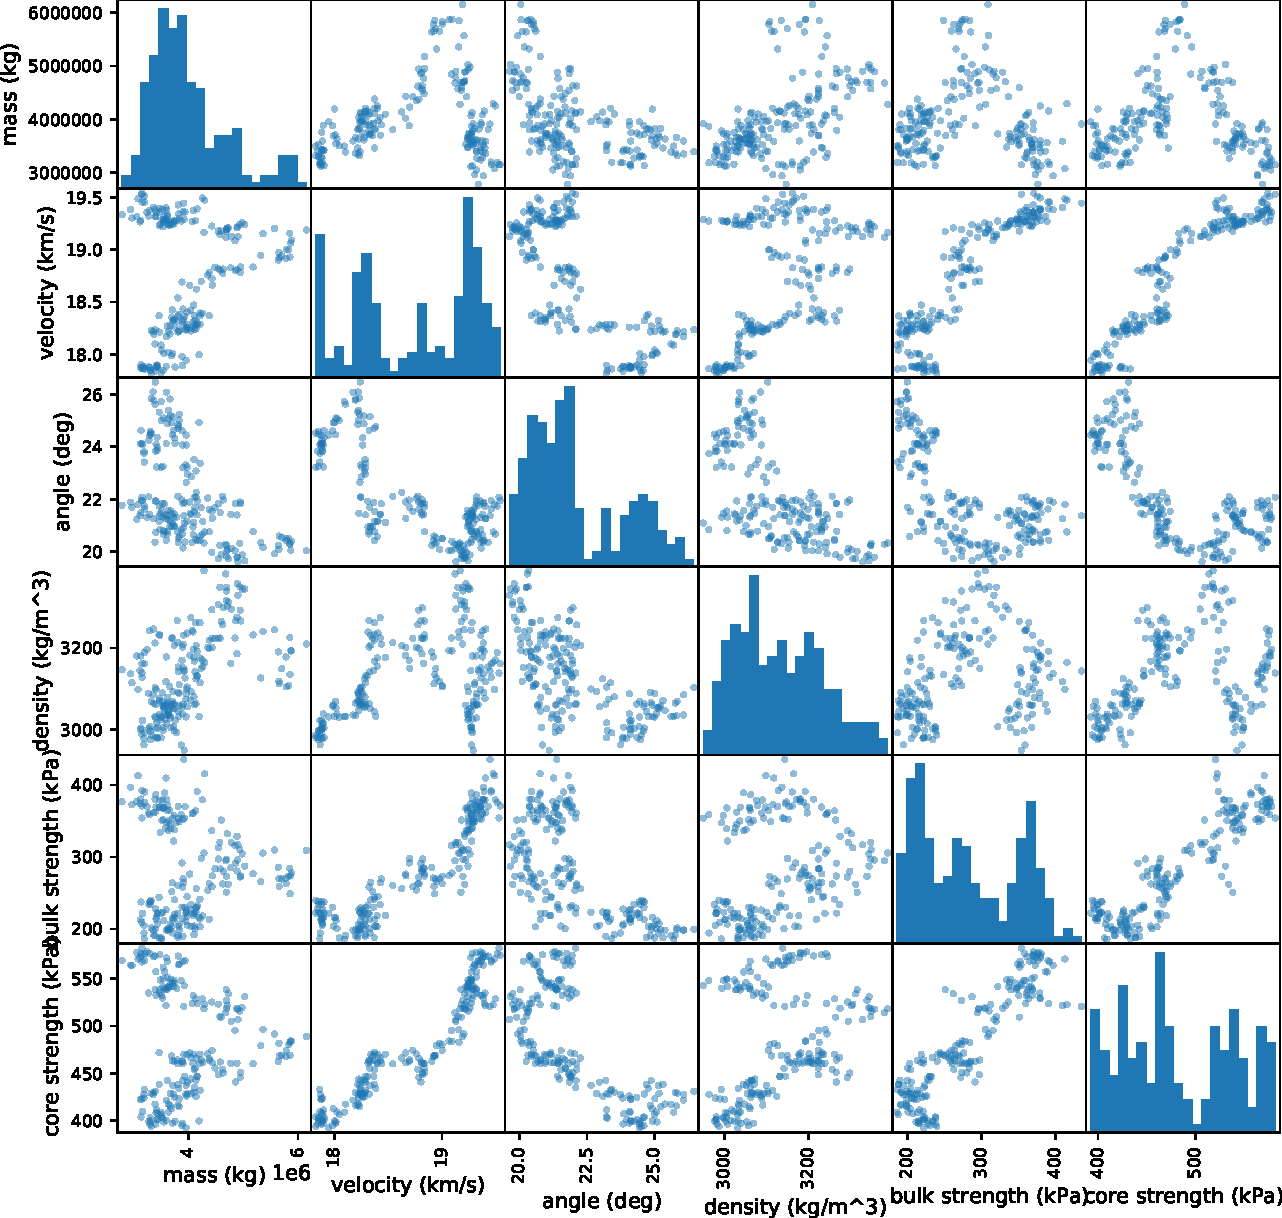
\includegraphics[width=\textwidth]{figures/posterior_ESP_038458_2030}
    \caption{Posterior distribution generated by our inversion algorithm from the observation with HiRISE ID ESP 038458 2030. We can see that the algorithm has not converged yet.}
    \label{fig:inversion_example_1}
\end{figure*}

\begin{figure*}
    \centering
    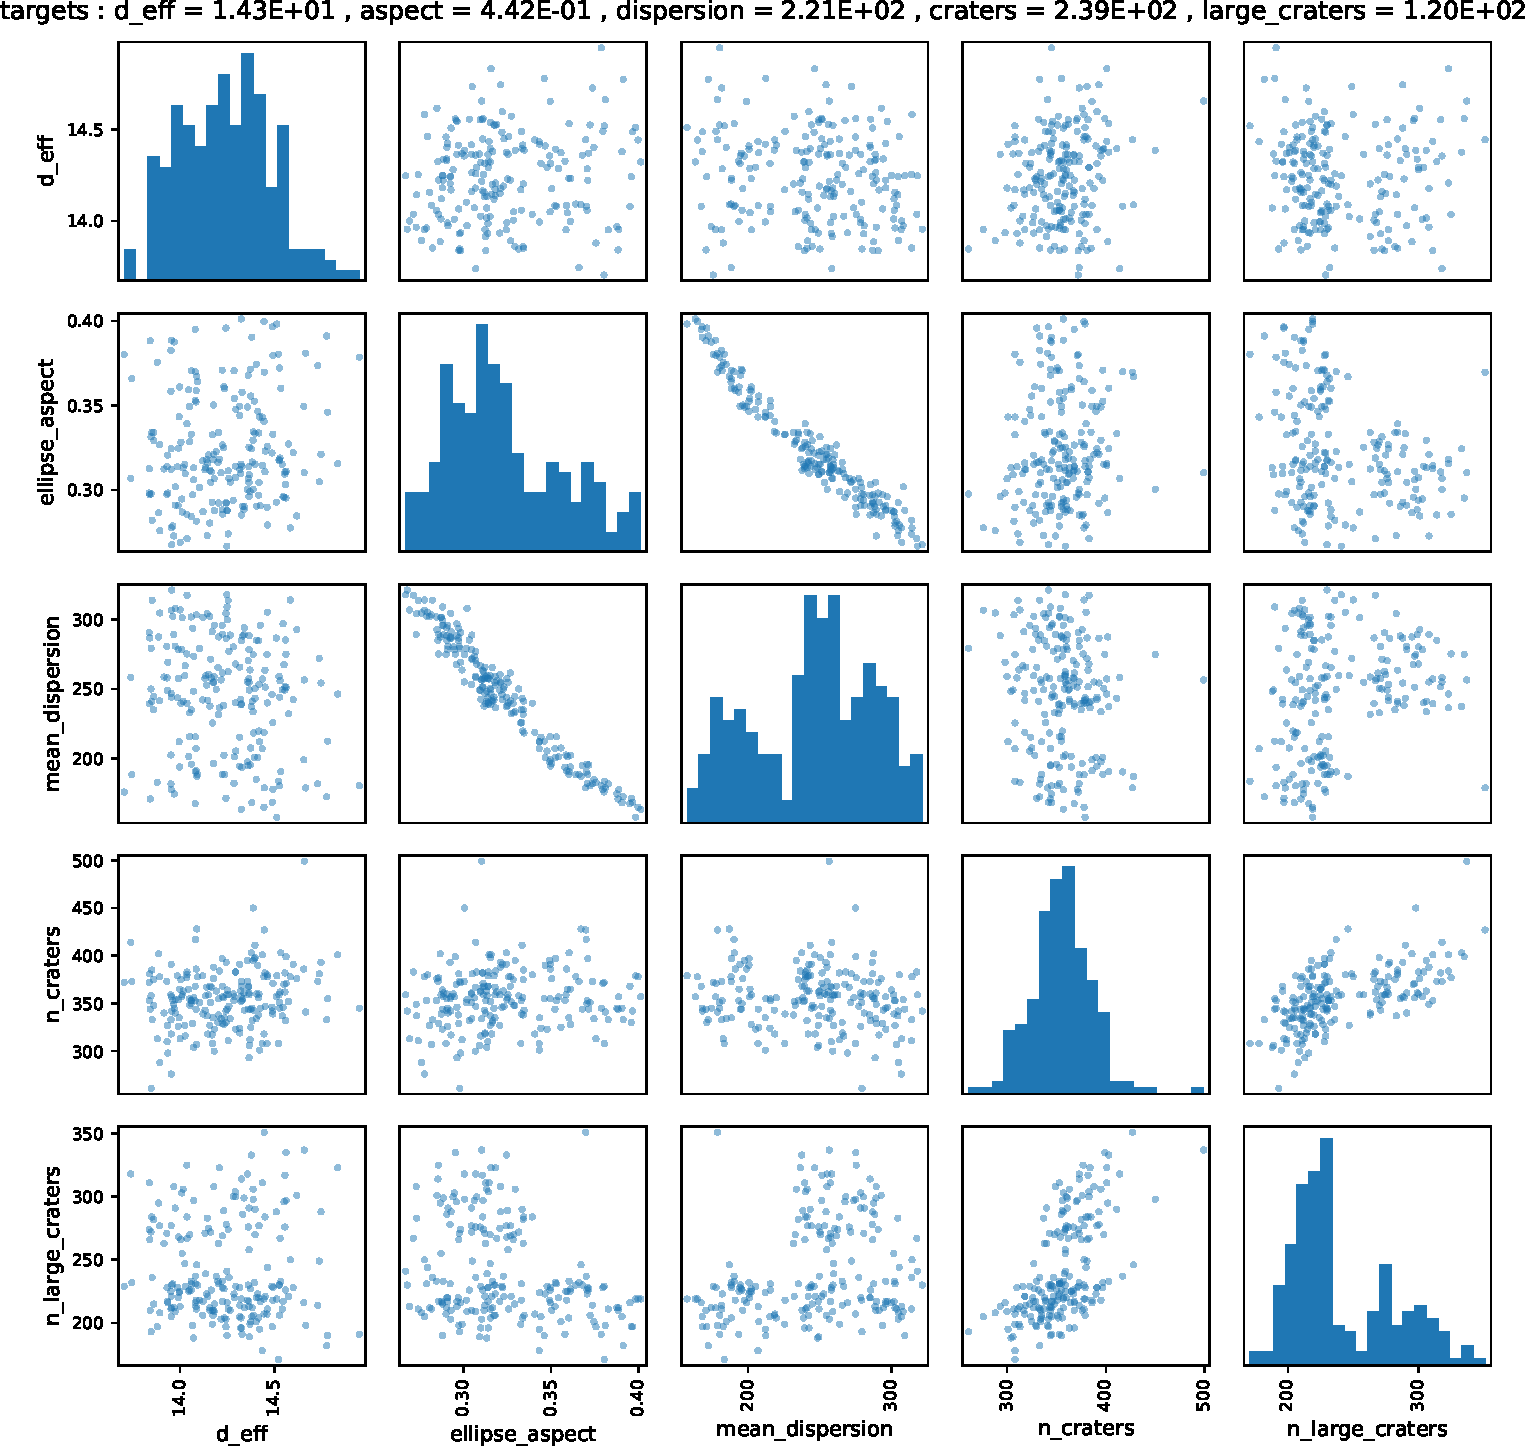
\includegraphics[width=\textwidth]{figures/characteristics_ESP_038458_2030}
    \caption{Cluster characteristics from the posterior distribution in fig.~\ref{fig:inversion_example_1}.}
    \label{fig:inversion_example_2}
\end{figure*}